% !TEX root = ../my-thesis.tex
%
\chapter{Technologien, Frameworks/Libraries, Programmiersprachen}
\label{sec:technologies}

\cleanchapterquote{Users do not care about what is inside the box, as long as the box does what they need done.}{Jef Raskin}{(US-Amerikanischer Informatiker, Experte für Mensch-Computer-Interaktion)}

In diesem Kapitel werden die für diese Arbeit verwendeten Technologien aufgelistet und beschrieben.
Zunächst wird das Konzept der \textit{\acl{PWA}} erklärt und erläutert welche Idee dahinter steckt. Dann werden mit Angular, React und Vue.js drei Frameworks beziehungsweise Libraries kurz vorgestellt und gleichermaßen deren Gemeinsamkeiten und Unterschiede als auch deren Vor- und Nachteile diskutiert. Anschließend wird begründet, warum die Wahl auf Angular gefallen ist und dieses Framework dann ausführlich beschrieben. Nach kurzer Vorstellung der Programmiersprache TypeScript, werden noch weitere Pakete und Materialien aufgelistet, welche für dieses Projekt verwendet wurden.

\section{Progressive Web Apps}
\label{sec:technologies:pwa}

Mobile Plattformen - also Smartphones und Tablet-PCs - haben in den letzten Jahren stark an Bedeutung gewonnen und auch wenn Desktop-PCs ihre Daseinsberechtigung in ein paar Jahren nicht verloren haben werden, so werden sie immer mehr als Werkzeug zum ``einfachen Surfen`` von wesentlich kompakteren Geräten abgelöst. Wer sich lediglich ein paar Informationen aus dem Internet beschaffen oder Dienstleistungen über dasselbe in Anspruch nehmen will, der kann dies viel einfacher mit einem Smartphone erledigen. Zudem hat man dieses heutzutage fast immer und überall dabei.

Auch wenn mit der steigenden Popularität solcher mobilen Geräte das \textit{Responsive Web Design}, bei dem sich das Layout einer Seite an das verwendete Geräte anpasst, immer wichtiger wurde, so waren \textit{Native Apps} zunächst das Mittel der Wahl, um Informationen auf mobilen Geräten darzustellen. Schließlich boten diese gegenüber den - zumindest in der Anfangszeit der Smartphones - eingeschränkten Funktionalitäten von mobilen Webbrowsern mehr Möglichkeiten und eine komfortablere Bedienung. Nachteil hierbei war (und ist), dass für die marktbeherrschenden Plattformen iOS von Apple und Android von Google auf Grund der unterschiedlichen Betriebssysteme unabhängige Versionen einer App entwickelt werden mussten; unter Umständen sogar noch für \textit{Windows Mobile} oder \textit{BlackBerry OS}, die allerdings beide in den letzten Jahren stark an Bedeutung verloren haben. Diese Mehrgleisigkeit  brachte also einen Aufwand mit sich, der umso lästiger war, wenn weiterhin eine responsive Webseite betrieben werden sollte, die als Erstanlaufstelle dient.

Eine Lösung dieses Problems bestand in der Entwicklung von  Werkzeugen, die es ermöglichen, eine App für mehrere Plattformen gleichzeitig zu entwickeln. Als Beispiel sei hier \textit{Xamarin}\cite{Xamarin} genannt, eine Sammlung von Werkzeugen, mithilfe derer Apps in der Programmiersprache C\# programmiert und diese dann für iOS, Android und Windows Phone exportiert werden können. Ein weiteres Beispiel ist das von \textit{Adobe} veröffentlichte Framework \textit{PhoneGap}\cite{Phonegapp}. Hierbei werden Apps im Prinzip als responsive Webseiten mit \acs{HTML}, \acs{CSS} und JavaScript entwickelt, die dann auf den Endgeräten in einer Art virtueller Maschine laufen. Der Vorteil dieses und vergleichbarer Frameworks liegt ganz offensichtlich darin, dass Webentwickler, die nie zuvor native Apps entwickelt haben, nach relativer kurzer Einarbeitungszeit in der Lage sind, Apps für verschiedene Plattformen zu programmieren.

Ein Haken bleibt bei der Verwendung von Tools wie Cordova aber bestehen: Mit solchen Frameworks entwickelte Apps müssen weiterhin über den \textit{Google Play Store} (im Falle von Android-Geräten), über den \textit{App Store} (für iOS-Geräte) oder die entsprechende Vertriebsplattform ausgeliefert und installiert werden. Das ist zum einen mit Lizenzauflagen für die Entwickler verbunden und kann zum anderen ein Hemmnis für Nutzer darstellen, die nicht für jede Kleinigkeit eine App auf ihrem Gerät installieren wollen.

Hier kommt das Konzept der \acf{PWA} ins Spiel. Dabei handelt es sich um Webseiten, die Funktionen und Vorteile von responsiven Webseiten und nativen Apps bzw. Desktopanwendungen kombinieren. Alex Russel, der zusammen mit Frances Berriman das Konzept der \acsp{PWA} ausgearbeitet hat nennt als Mindestanforderung die folgenden Kriterien: \cite{PWA}

\begin{itemize}  
\item Sie funktionieren (zumindest eingeschränkt) auch ohne Internetverbindung.
\item Sie werden über eine sichere Verbindung (also via HTTPS) ausgeliefert.
\item Sie enthalten ein \hyperref[sec:technologies:pwa:manifest]{Manifest}, dass bestimmte Eigenschaften der Webseite angibt.
\end{itemize}

Diesen Hauptkriterien müssen erfüllt sein, damit kompatible Browser den Benutzer zum Installieren der Webseite als Desktop- oder Mobile-App auffordern können. Darüber hinaus gibt es wünschenswerte Kriterien, wie zum Beispiel, dass \acsp{PWA} möglichst schnell laden oder von Plattform und Browser unabhängig sind. Dabei heißt ```schnell laden`` nicht zwangsläufig, dass die ganze Seite geladen worden ist, sondern das möglichst schnell ein rudimentärer Inhalt angezeigt wird, sodass der Nutzer eher geneigt ist etwas länger zu warten, bis die Seite dann vollständig aufgebaut wurde.

Eine \acs{PWA} muss zu den eigentlichen HTML-, JavaScript- und CSS-Dateien noch eine Manifest-Datei und eine JavaScript-Datei, in welcher der ``Service Worker`` implementiert wird, enthalten. In der Manifest-Datei werden bestimmte Eigenschaften angegeben und über den Service Worker werden die Funktionalitäten implementiert, welche eine \acl{PWA} von einer normalen Webseite unterscheiden. Beides wird im Folgenden vorgestellt und erläutert.

\subsection{Manifest}
\label{sec:technologies:pwa:manifest}
Bei der Manifest-Datei handelt es sich um eine Datei im \acs{JSON}-Format, in der mindestens folgende Eigenschaften der \acs{PWA} definiert werden müssen:\cite{Manifest}

\begin{itemize}
\item Der Name der Web App (in Langform)
\item Web App-Name in Kurzform für die Beschriftung der Verknüpfung
\item Der Wurzelpfad der Webseite (damit bei ``Installation`` der \acs{PWA} nicht der aktuelle Pfad als Link gespeichert wird)
\item Die Art, wie die ``installierte`` Seite geöffnet werden soll: in einem normalen Browser-Fenster, in einem Browser-Fenster mit minimalen Steuerelementen, als eigenständige Anwendung in einem normalen Fenster oder im Vollbildmodus.
\item Eine Liste von Icons für die Verknüpfung: typischerweise wird das Icon in mehreren Auflösungen hinterlegt, damit es auch auf hochauflösenden Geräten vernünftig dargestellt wird
\end{itemize}

Zusätzlich können hier Attribute definiert werden, wie Farbe für Hintergrund, sowie Fenster und Taskleiste auf Android-Geräten, Sprache und Leserichtung des Namens in Kurz- und Langform oder ein ``Scope``, der angibt, welche Seiten zur \acl{PWA} gehören und welche in einem normalen Browserfenster geöffnet werden sollen.


\subsection{Service Worker}
\label{sec:technologies:pwa:sw}

Die Hauptaufgabe des Service Worker besteht darin, Anfragen nach Ressourcen (Skripte, CSS-, XML-, JSON- oder sonstige Dateien), die eigentlich an einen Server geschickt werden sollen, abzufangen, und stattdessen im Cache gespeicherte Versionen der Dateien zu verwenden. Hierbei ist zu konfigurieren, welche Ressourcen überhaupt im Cache gespeichert werden sollen, wie lange sie dort maximal gespeichert werden dürfen, bevor sie als veraltet zu betrachten und durch neuere Versionen zu ersetzten sind, und wie viel Speicherplatz der Cache maximal belegen darf. Damit diese Funktionen genutzt werden können muss - nachdem beim Seitenaufruf alle Ressourcen geladen worden sind - überprüft werden, ob der verwendete Browser die Service Worker-\acs{API} überhaupt unterstützt. Ist dies der Fall, kann das Skript, in dem der eigentliche Service Worker implementiert wird, registriert werden.

Durch das Speichern der Ressourcen im Cache kann die Webseite dann auch aufgerufen werden, wenn keine Internetverbindung vorhanden ist. Aber auch mit Internetverbindung ist so ein großer Performance-Gewinn möglich; eine Seite kann dann quasi augenblicklich geladen werden, weil auf lokal gespeicherte Ressourcen zurückgegriffen werden kann, statt auf die Antwort eines Servers warten zu müssen. Das kann vor allem auf Mobilgeräten von Vorteil sein, wenn nur eine schwache Mobilfunkverbindung verfügbar ist\cite{ServiceWorker}.

Zudem können über den Service Worker sogenannte Push-Benachrichtigungen implementiert werden, da dieser immer im Hintergrund aktiv ist. Somit können die Benutzer über Neuigkeiten informiert werden, wie es auch bei nativen Anwendungen und Apps möglich ist. Es kommt sogar häufig vor, dass ein Service Worker nur für solche Benachrichtigungen genutzt und gar keine Daten im Cache gespeichert werden.

Außerdem unterstützt der Service Worker sogenanntes ``Background Sync``. Hierbei werden Daten, die an einen Server geschickt werden sollen, bei nicht vorhandener Internetverbindung gespeichert und sobald eine Verbindung wiederhergestellt wurde, dann versendet.

Geplant ist darüber hinaus, dass Service Worker in Zukunft auch periodisches Synchronisieren unterstützen, sodass in Intervallen, zu bestimmten Zeiten aber auch in Abhängigkeit des Akkuladestandes oder der Art der Netzwerkverbindung eine Kommunikation zwischen Server und Webanwendung erfolgt. Hierzu gibt es allerdings noch keine offizielle Spezifikation\cite{SwFuture}.

\subsection{Kompatibilität}
Zwar sind \aclp{PWA} prinzipiell ``nur`` Webseiten und als solche im Allgemeinen nicht vom Endgerät abhängig, aber noch unterstützen nicht alle Browser auf allen Plattformen die Technologie der Service Worker und auch die Manifest-Datei einer \acs{PWA} wird noch von einigen Browsern (zumindest auf manchen Plattformen) ignoriert. Während sowohl auf Geräten mit den Betriebssystemen Windows 10, Android oder einer Linux-Distribution \acsp{PWA} von den dort verfügbaren Browsern fast vollumfänglich unterstützt werden, gibt es auf Geräten mit dem Apple-Betriebssystemen iOS noch teils erhebliche Einschränkungen. Lediglich der Apple-eigene Safari-Browser unterstützt auf dieser Plattform die Service Worker-Technologie, aber selbst hier sind keine Push-Benachrichtigungen und keine Hintergrundaktualisierungen möglich.
Auf MacOS-Geräten ist die Unterstützung des Safari-Browsers ähnlich schwach, allerdings sind sowohl Chrome als auch Opera (bis auf das Installieren als Desktop-Anwendung) vollständig kompatibel.\cite{Compatibility}

\section{Frameworks und Libraries: Angular, React und View}
\label{sec:technologies:frameworks}

Beim Entwickeln von Software jeglicher Art sind Frameworks und Libraries weitverbreitete Hilfsmittel, um nicht jede einzelne Funktion neu programmieren zu müssen, sondern auf vorhandene Komponenten zurückgreifen zu können, sodass viel Arbeit gespart werden kann. Auch wenn die Bezeichnungen ``Framework`` und ``Library`` vor allem im Bereich der Webentwicklung häufig synonym verwendet werden, kann man doch differenzieren, was die Funktions- bzw. Verwendungsweise betrifft. Allgemeiner Konsens ist: Eine \textit{Library} wird verwendet, um Lücken in der eigenen Anwendung zu schließen, während man bei Verwendung eines \textit{Frameworks} die Lücken desselben füllen muss. Genauer bedeutet dies, dass man die Funktionen einer Library in der eigene Anwendung aufrufen muss, während man bei einem Framework den eigenen Code in ein vorgegebenes Grundgerüst einbinden muss\cite{FrameVsLib}.

Im Folgenden werden mit Angular, React und Vue drei derzeit sehr populäre Frameworks/Libraries vorgestellt und miteinander verglichen\cite{AngularReactVue} und anschließend begründet, warum Angular für dieses Projekt verwendet wird. Bei allen drei handelt es sich dabei um unter MIT-Lizenz veröffentlichte \textit{Open Source}-Software, die zum Programmieren von Benutzerschnittstellen konzipiert ist. Außerdem sind alle drei ``komponentenbasiert``; man entwickelt \textit{Components}, die als Bausteinen dienen, um damit eine Webseite aufzubauen.

\subsection{Angular}
\label{sec:technologies:frameworks:angular}
Das von Google entwickelte Framework erschien ursprünglich im Oktober 2010 unter dem Namen ``AngularJS``; mit der Veröffentlichung der Version 2.0.0 im September 2016, die eine grundlegende Überarbeitung mit sich brachte, wurde der Name in ``Angular`` geändert, um sich klar von den alten Versionen zu distanzieren, schließlich sind diese nicht miteinander kompatibel\cite{AngularNaming}.

Während AngularJS in JavaScript geschrieben wurde, basiert Angular auf der von Microsoft entwickelten Programmiersprache TypeScript. Diese Programmiersprache wird in Kapitel \ref{sec:technologies:ts} kurz vorgestellt. Verwendet man also Angular empfiehlt es sich, in TypeScript zu programmieren, auch wenn es grundsätzlich möglich ist, weiterhin JavaScript zu nutzen. Die offizielle Dokumentation beschränkt sich allerdings auf die Verwendung von TypeScript. Angular baut auf der in JavaScript programmierten \textit{NodeJS}-Serverumgebung auf und benötigt den Paketverwaltungsmanager \textit{npm}, mit welchem dem Projekt ganz einfach weitere Softwarepakete hinzugefügt werden können.

Ein Nachteil von Angular ist, dass es relativ umständlich und schwierig ist, mit diesem Framework entwickelte Komponenten in eine bestehende Webseite einzufügen. Während es durchaus Anleitungen gibt, welche beschreiben wie das möglich ist, beschränkt sich die offizielle Dokumentation darauf, zu erklären, wie mit Angular \textit{\acfp{SPA}} erstellt werden können.  Außerdem ist Angular auch zu umfangreich, als dass es sinnvoll wäre, dieses Framework ``nur`` für ein paar Komponenten zu einer bestehenden Webseite hinzuzufügen. Es einfach eher dafür konzipiert, eigenständig verwendet zu werden. Allerdings ist es durchaus möglich, eine Angular-Web-App in einem Unterverzeichnis einer bestehenden Webseite einzubinden - dann aber wieder als in sich geschlossene Einheit.

Auch wenn Angular an sich schon relativ komplex und umfangreich ist - was sich auch auf die Dokumentation des Frameworks auswirkt -, können mit dem \textit{ng add}-Befehl des Angular-\acs{CLI} ganz einfach neue Pakete und Funktionalitäten hinzugefügt werden. Das  Angular-\acs{CLI} wurde mit Version 2.0.0 von Angular eingeführt, ist aber nicht fester Teil von Angular, sondern muss manuell installiert werden. Mit diesem \acl{CLI} können u.a. die verschiedenen Komponenten von Angular generiert werden, aber auch ein Testserver mit \textit{ng serve} gestartet oder mit \textit{ng build} der \textit{Build-Prozess} initiiert werden \cite{AngularCLI}. Eine ausführlichere Beschreibung erfolgt in Kapitel \ref{sec:technologies:angular:cli}.

Vorteilhaft sind die vom Entwicklerteam von Angular selbst verwalteten Pakete wie der Router oder der \acs{HTTP}-Client zur Kommunikation mit einer \acs{API}, die bei anderen Frameworks oder Libraries von Drittquellen bezogen werden müssen. Dadurch kann eine höhere Stabilität und Sicherheit gewährleistet werden und bei Updates gibt es keine Kompatibilitätsprobleme. Weitere Details und Eigenschaften von Angular werden in Kapitel \ref{sec:technologies:angular} erläutert.

\subsection{React}
\label{sec:technologies:frameworks:react}

Mit Facebook steht hinter React ebenfalls ein großes Unternehmen; bei diesem Projekt handelt es sich jedoch um eine \textit{Library}. Diese wurde erstmalig im Mai 2013 veröffentlicht und kann - im Gegensatz zu Angular - ganz einfach zu bestehenden Projekten hinzugefügt werden. Es wurde aber auch schon vor der Veröffentlichung von Facebook selbst seit 2011 genutzt. Zwar wird auch hier ein komponentenbasierter Ansatz verfolgt, allerdings sind die Komponenten bei React oftmals kleiner und nicht so umfangreich, da sie lediglich einzelne Elemente repräsentieren. Wie bei Angular können auch bei React Komponenten ineinander verschachtelt werden.

React verwendet \acf{JSX}, eine Erweiterung von JavaScript, bei der im Prinzip HTML-Code in Javascript-Code eingebettet wird\cite{ReactJSX}. Im Gegensatz dazu werden bei Angular die \textit{HTML-Templates} von Komponenten in der Regel in eigene Dateien ausgelagert (siehe Kapitel ref{sec:technologies:angular:component:html}), was bei größeren \textit{Templates} von Vorteil ist.
und auch dem Konzept des \textit{Separation of Concerns} entspricht. Allerdings sind Komponenten in der Regel so gestaltet, dass deren Template überschaubar ist.
\begin{lstlisting}[float, floatplacement=h, style=htmlcssjs, caption={Code-Beispiel für React mit einem \textit{Functional Component}}, label={React}]
function Welcome(props) {
  return <h1>Hello, {props.name}</h1>;
}

const element = <Welcome name="Sara" />;
ReactDOM.render(
  element,
  document.getElementById('root')
);
\end{lstlisting}
Anders als Angular ist React nicht abhängig von \textit{NodeJs} oder \textit{npm}. Es gibt aber dennoch ein \acs{CLI}-Paket, das über \textit{npm} bezogen werden kann, mit dem unter anderem ein neues Projekt erzeugt oder dieses für die Auslieferung ``gepackt`` werden kann\cite{ReactCli}.

Diese Library ist nicht so komplex wie Angular, dementsprechend ist auch die Lernkurve weniger steil. Da diese Library eher für das Erstellen von Benutzer-Interfaces gedacht ist, fehlen Funktionalitäten wie z.B. ein Router zum Navigieren zwischen ``virtuellen Seiten`` oder ein \acs{HTTP}-Client. Dafür gibt es dann Pakete aus einer aktiven Community, die diese Features nachliefern.

Ein weiterer Unterschied zu Angular ist der, dass diese Library ganz einfach zu einer bestehenden Webseite hinzugefügt werden kann, indem der Quellcode von React und ReactDOM (über das die Manipulation des \acf{DOM} geregelt wird) mittels \textit{Script}-Tag in das \acs{HTML}-Dokument eingebunden wird. Dann können Komponenten in einer oder mehreren JavaScript-Dateien implementiert werden\cite{ReactAdd}.

Anders als Angular verwendet React das Konzept des sogenannten \textit{Virtual \acs{DOM}}. Hierbei wird ein virtuelles Abbild des eigentlichen \acsp{DOM} erzeugt und bei Änderung von Daten des zugrunde liegenden Modells bestimmt, welche Teile des \acsp{DOM} aktualisiert werden müssen. Da es sich bei dem \acs{DOM} um eine Datenstruktur in Form eines Baumes handelt, ist das Durchsuchen eines solchen zwar relativ schnell möglich, das Aktualisieren und Umstrukturieren kann aber mitunter sehr aufwändig sein. Mit Hilfe des Virtual DOMs sowie eines speziellen Algorithmus kann React diese Prozedur beschleunigen\cite{VirtualDom}.

\begin{lstlisting}[float, floatplacement=h, style=htmlcssjs, caption={Code-Beispiel für ein \textit{Class Component} bei React}, label={ReactAltern}]
class Welcome extends React.Component {
  constructor() {
	/* Initialisierungen */  
  }
  render() {
    return <h1 onClick={() => this.handleClick()}>Hello { this.props.name }</h1>
  }
  handleClick() {
    /* Auf 'Klick' reagieren */
  }
}

const element = <Welcome name="Sara" />;
ReactDOM.render(element, document.getElementById('root'));
\end{lstlisting}
Im Code-Beispiel \ref{React} wird gezeigt, wie eine simple React-Komponente aussehen kann\cite{ReactComponent}. Das in Zeile 5 definierte Element wird beim \textit{rendern} der Seite als Kindelement des \acs{DOM}-Elements mit der ID 'root' in das DOM eingebunden (Zeile 6). Dadurch, dass als Wert des \textit{name}-Attributes des Elements ``Sara`` festgelegt wurde, bekommt die Seite also die Überschrift ``Hello, Sarah``. In Zeile 1-3 ist ein Beispiel für \textit{JSX} geben; JavaScript und HTML werden hier miteinander vermischt. Soll die Komponente zusätzliche Funktionen besitzen, um beispielsweise das Anklicken dieser zu verarbeiten, so würde man eine Klasse definieren, die von \textit{React.Component} ``erbt``. Das \textit{return-Statement} würde dann in eine \textit{render}-Methode verschoben. Code-Beispiel \ref{ReactAltern} zeigt, wie das aussehen kann. Entscheidend ist hier die \textit{render}-Methode, die definiert sein muss, weil sie aufgerufen wird, wenn die Komponente ins \acs{DOM} eingebunden werden soll und daher als Rückgabe ein Template liefern muss.

\subsection{Vue.js}
\label{sec:technologies:frameworks:view}

Zwar handelt es sich bei Vue.js (gesprochen wie ``view``) wie bei Angular um ein Framework, dieses kann jedoch im Gegensatz zu Angular ohne große Probleme in bestehende Webseiten bzw. Webanwendungen eingebunden werden. Das funktioniert analog zur Vorgehensweise von React.
Vue.js ist, vor allem im Vergleich mit Angular, sehr kompakt und deswegen besser geeignet, wenn lediglich ein paar interaktive, dynamische Elemente ergänzt werden sollen.

Anders als bei React und Angular steht hinter diesem Projekt kein großes Unternehmen, sondern ein vergleichsweise kleines Team. Erstmalig veröffentlicht wurde diese Library im Februar 2014\cite{Vue}. Damit ist Vue.js, das zunächst vom ehemaligen Google-Mitarbeiter Evan You alleine entwickelt wurde - auch heute noch leitet er das Projekt -, jünger als Angular und React. Aufgrund des kleinen Entwicklerteams und weil es noch nicht ganz so alt ist, ist diese Library jedoch noch nicht ganz so umfangreich. Während zum Beispiel wie bei React ein HTTP-Client fehlt, gibt es bei Vue.js ein offizielles Routing-Paket. Ähnlich wie bei React gibt es auch hier eine sehr aktive Community, die eigene Pakete entwickelt, sodass das Framework bei Bedarf um weitere Funktionalitäten erweitert werden kann. Eine weitere Gemeinsamkeit von React und Vue.js ist die Verwendung eines \textit{Virtual \acs{DOM}}.

Wie eine Komponente bei Vue.js definiert werden kann, ist in Beispiel \ref{VueComponent} dargestellt\cite{VueComponent}. Hier wird eine Vue-Komponente erzeugt, deren Template jedes \acs{DOM}-Element mit dem Tag-Namen ``heading`` ersetzt. Das funktioniert allerdings erst, wenn wie hier in Zeile 8 ein \textit{Scope} definiert wird. Sollte es außerhalb des Elements mit der ID ``app`` Elemente mit dem Tag-Namen ``heading`` geben, werden diese nicht ersetzt.

\begin{lstlisting}[float, floatplacement=h, style=htmlcssjs, caption={Code-Beispiel für ein \textit{Component} in Vue.Js}, label={VueComponent}]
Vue.component('heading', {
  data: function() {
    [...]
    return {name: user.name};
  },
  template: '<h1>Wilkommen, {{ name }}</h1>'
});
new Vue({el: '#app'});
\end{lstlisting}
Bei großen Projekten bzw. komplexen Komponenten empfiehlt es sich, sogenannte \textit{Single File Components} zu verwenden. Hierbei wurde einen Zwischenweg von Angular und React gewählt: Sowohl Template- als auch Skript-Code befinden sich in einer Datei mit der Endung .vue , jedoch werden diese beiden nicht wie bei der \acs{JSX}-Syntax von React miteinander vermischt. Stattdessen stehen in einer .vue-Datei der Template-Code und der JavaScript-Code (alternativ auch TypeScript-Code) in getrennten Abschnitten und es können noch \acs{CSS}-Regeln, die nur für diese Komponente gelten, ergänzt werden. Diese Abschnitte werden durch \acs{XML}-artige Tags ausgezeichnet. Durch die Nutzung dieses speziellen Datei-Typs sind IDEs zudem in der Lage, besseres \textit{Syntax-Highlighting} zu liefern. Das Code-Beispiel  \ref{VueSFC} zeigt, wie eine solche Datei aussehen kann. Will man allerdings solche \textit{Single File Components} verwenden, dann ist man auf \textit{Webpack} angewiesen, mit dem die einzelnen Dateien in einer einzigen zusammengefasst werden. Dieses Werkzeug ermöglicht generell das Aufteilen von Code in Module, die dann vor dem Ausliefern gebündelt werden und wird ebenfalls von Angular verwendet.

\begin{lstlisting}[float, floatplacement=h, style=htmlcssjs, caption={Code-Beispiel für ein \textit{Single File Component} in Vue.Js}, label={VueSFC}]
<template>
  <h1>Wilkommen, {{ name }}</h1>
</template>
<script>
/*...*/
module.exports = {
  data: function() {
  /*...*/
    return { name: user.name };
  }	
}
</script>
<style>
h1 {
  color: blue;	
}
</style>
\end{lstlisting}
Die Reihenfolge der Abschnitte ist dabei egal, es ist allerdings empfehlenswert, in allen Dateien die gleiche Reihenfolge beizubehalten\cite{VueSFC}.

\subsection{Warum Angular}
\label{sec:technologies:frameworks:why}

Entscheidet man sich bei der Entwicklung eines Projektes für die Verwendung eines Frameworks oder einer Library, so können mehrere Faktoren für die Wahl wichtig sein. Generell sollte man sich überlegen, wie groß der Anteil der genutzten Funktionalitäten ist und ob sich auf Grund dessen der Einsatz überhaupt lohnt. Insbesondere sollte der Mehraufwand, welcher durch die Verwendung eines Frameworks entsteht, in einem vernünftigen Verhältnis zum eigentlichen Projektumfang stehen. Bei der Wahl eines Frameworks sollte man im Hinterkopf behalten, dass man sich einer (oftmals) starren Struktur fügen muss, während man bei einer Library in der Regel flexibler arbeiten kann. Weiterhin ist ein Abgleich der an das Projekt gestellten Anforderungen und den vom Framework bzw. der Library angebotenen Möglichkeiten sinnvoll.

Ein weiteres Kriterium auf das man bei der Auswahl Wert legen kann, ist die Popularität. Je weiter verbreitet ein Framework oder eine Library ist, desto einfacher ist es, bei Schwierigkeiten Hilfe in entsprechenden Foren zu bekommen und umso wahrscheinlicher ist es, dass bereits jemand das selbe Problem hat oder hatte. Außerdem gibt es bei populäreren Projekten auch mehr zusätzliches Material zur Einarbeitung. Weiterhin kann es auch von Vorteil sein, wenn ein Framework oder eine Library von einem größeren Unternehmen entwickelt wird, weil dieses zum einen schneller bestehende Fehler beseitigen kann und zum anderen eine gewisse Zukunftssicherheit mit sich bringt: Während es bei ``Ein-Mann-Projekten`` durchaus passieren kann, dass dieses quasi unvermittelt eingestellt wird, ist das bei populären Frameworks und Libraries, hinter denen eine größere Firma steht, eher unwahrscheinlich.

Auch wenn Angular recht komplex und umfangreich ist und zudem auch eine Einarbeitung in die Programmiersprache TypeScript notwendig bzw empfehlenswert ist, gibt es dennoch überzeugende Gründe, welche für dieses Framework sprechen. Zunächst einmal ist es von Vorteil, dass Angular einen \acs{HTTP}-Client mitbringt, der für die Nutzung der verschiedenen \acsp{API} notwendig ist. Weiterhin ist Angular für die Entwicklung von \acsp{SPA} durch das ebenfalls vom Angular-Entwicklerteam gepflegte \textit{Router}-Paket prädestiniert. Dies ist zwar keine zwingende Anforderung an die zu entwickelnde Webanwendung, es ist allerdings einfacher, eine \acl{SPA} als \acl{PWA} umzusetzen als eine herkömmliche Webseite, da unter anderem weniger HTML-Dokumente im Cache gespeichert werden müssen. Außerdem soll sich eine \acs{PWA} möglichst schnell anfühlen, was mit einer \acs{SPA} erreicht wird, indem nur Teile einer Webseite neu geladen werden (mehr dazu in Kapitel \ref{sec:technologies:angular:routing}). Bei React wird mehr Wert darauf gelegt eine Möglichkeit zu bieten, interaktive und dynamische Elemente zu einer Seite hinzufügen zu können; Router und HTTP-Client,  gibt es beide nur aus Dritt-Quellen. Die Entwickler von Vue.js bieten zumindest ein offizielles Routing-Paket an.

Darüber hinaus kann mit dem vom Angular-Team entwickelten Paket \textit{@angular/pwa} mit dem Angular-\acs{CLI}-Befehl \textit{ng add} einem Projekt hinzugefügt werden, sodass aus diesem ganz einfach eine \acl{PWA} gemacht wird - eine Kernanforderung dieses Projekts.

\section{Das Angular-Framework im Detail}
\label{sec:technologies:angular}

In diesem Kapitel wird das Angular-Framework und seine Funktionsweise detaillierter vorgestellt. Dabei wird auch erklärt, aus welchen Bausteinen eine mit Angular entwickelte Web-Anwendung besteht und welche Funktion(en) diese erfüllen. Sämtliche Beschreibungen beziehen sich hierbei auf die Verwendung von TypeScript. Darüber hinaus können natürlich auch Klassen oder Interfaces implementiert werden, bei denen es sich nicht um Angular-spezifische Elemente handelt, sondern um solche, die dem Modellieren und Verarbeiten der empfangenen oder zu sendenden Daten dienen.

Abgesehen von einem generell notwendigen \textit{HTML}-Dokument, typischerweise mit dem Dateinamen \textit{index.html}, und sonstigen \textit{Stylsheets} oder Skripten (Analytics, Werbeanzeigen etc.) besteht eine Angular-Web-App mindestens aus einem \textit{ngModule} (vgl Kapitel \ref{sec:technologies:angular:module}) und einem \textit{Component}.


\subsection{Components}
\label{sec:technologies:angular:component}
Sogenannte \textit{Components} - also Komponenten - sind die Hauptbausteine einer jeden Angular-Web-App. Eine solche Komponente kann ein rechtes einfaches Element wie Textbausteine (vergleichbar mit \textit{div}- oder \textit{p}-Tags) sein, Bedienelemente wie Buttons oder Textfelder repräsentieren, aber auch aus mehreren solcher Elemente zusammengesetzt und damit quasi eine ganze Seite repräsentieren. Streng genommen bezieht sich der Ausdruck ``Component`` dabei auf eine spezielle Klasse, zu der ein \acs{HTML}-Template gehört, welches über Attribute und Methoden der Klasse manipuliert werden kann. Da das Template Teil des \acsp{DOM} ist, ändert sich damit auch die Seite. Außerdem kann eine Komponente auch aus anderen Komponenten zusammengesetzt sein. Eine Komponente muss dabei immer Teil eines Moduls sein, also im \textit{imports}-Array eines Moduls auftauchen - dazu mehr in Abschnitt \ref{sec:technologies:angular:module}.

\subsubsection{\textit{Komponente}.component.ts}
\label{sec:technologies:angular:component:ts}
Definiert wird eine Komponente in einer Datei mit der Endung ``.component.ts``, wobei die Dateiendung \textit{.ts} für TypeScript steht. Die Hauptkomponente, welche die ganze Web-App umfasst, wird beispielsweise standardmäßig in einer Datei mit dem Namen \textit{app.component.ts} implementiert.

Der Code-Ausschnitt \ref{AppComponent} zeigt, wie eine solche Datei aufgebaut ist. Zunächst erfolgen die Importe von notwendigen Modulen, Komponenten/Direktiven, und Services. Danach folgt der \textit{Decorator}, durch den festgelegt wird, dass die anschließend implementierte Klasse ein \textit{Component} ist, in dem aber auch verschiedene \textit{Optionsmetadaten} definiert werden (können). Die wichtigsten davon sind:

\begin{itemize}
\item \textbf{selector}: Dieser CSS-Selektor gibt das \acs{DOM}-Element an, zu dem das Template der Komponente als Kindelement hinzugefügt werden soll. 
\item \textbf{template/templateUrl}: Hier wird das zugehörige Template bzw. ein Pfad zu einer Datei, in der das Template definiert ist, angegeben.
\item \textbf{style/styleUrls}: Die CSS-Regeln für das Design der Komponente bzw. ein Liste von Pfaden zu CSS-Dateien für diese Komponente werden hier aufgelistet.
\end{itemize} 

Außerdem können Services, die von dieser Komponente genutzt werden, angegeben werden, falls dies nicht schon in einem übergeordneten Modul organisiert wird. Anschließend wird die eigentliche Klasse der Komponente angegeben. Damit diese an anderer Stelle \textit{importiert} werden kann, muss sie hier auch \textit{exportiert} werden. Das ist allerdings keine Eigenheit von Angular, sondern unterliegt der generellen Funktionsweise von JavaScript beziehungsweise TypeScript.

\begin{lstlisting}[float, floatplacement=h, style=htmlcssjs, caption={Bespiel für eine \textit{AppComponent}.ts-Datei}, label={AppComponent}]
//Importe anderer Module/Komponenten/...
import {Component, OnInit} from '@angular/core';

@Component({
  selector: 'app-root',
  templateUrl: './app.component.html',
  styleUrls: ['./app.component.css']
})
export class AppComponent implements OnInit {
	//Klassenvariablen
	heading = 'Wilkommen';
	names = ['Alice, Bob, Charlie'];

  constructor() {  }

  ngOnInit() {
    // Initialisierungen
  }
}
\end{lstlisting}
Typischerweise gibt es in der Klasse der Komponente eine Funktion \textit{ngOnInit}, über welche die Initialisierung der Instanz der Komponente vorgenommen wird. Zum Beispiel können Daten von einem Server angefragt werden, um sie dann in die Komponente zu integrieren. Zwar kann auch eine \textit{constructor}-Methode angegeben werden, diese ist allerdings hauptsächlich für \textit{Dependency Injection} zuständig, also das Einbinden von Objekten, die nicht vom einbindenden Objekt selbst instanziiert werden. Ansonsten werden, wie bei objektorientierter Programmierung üblich, Instanzvariablen und Methoden definiert\cite{ComponentTS}.

\subsubsection{\textit{Komponente}.component.html}
\label{sec:technologies:angular:component:html}

\begin{lstlisting}[float, floatplacement=h, style=htmlcssjs, caption={Beispiel für eine index.html-Datei einer Angular-App}, label={IndexHTML}]
<!doctype html>
<head>
<!--Meta-Tags, Stylesheets, Skripte...-->
</head>
<body>
  <app-root>
  	<!-- Die Templates der Komponenten werden hier eingesetzt -->
  </app-root>
  <noscript>
    Du musst JavaScript aktiviert haben, um diese Seite zu verwenden.
  </noscript>
  <!-- Autmatisch generierte Skript-Dateien werden hier eingebunden -->
</body>
\end{lstlisting}

Ist das \textit{Template} der Komponente zu groß, wird es der Übersicht halber ausgelagert in eine Datei mit der Endung \textit{.component.html}. Mittels \textit{Two-Way Data Binding} kann bei Angular das \acs{DOM} mit einer Komponente verknüpft werden, sodass sich das ersteres ändert, wenn sich die Komponente bzw. der Wert einer Instanzvariablen der Komponente ändert und umgekehrt.

Der \textit{selector} im in Code-Ausschnitt \ref{AppComponent}, deutet an, dass es sich dabei um das \textit{Root Component} - also die Wurzelkomponente -  handelt, welche als Container für die ganze Web-App dient. Dieser Selektor bezieht sich auf ein \acs{HTML}-Element mit dem Tag-Namen ``app-componenent`` wie zum Beispiel in Zeile 6 in Beispiel \ref{IndexHTML}. Innerhalb dieses Elements wird dann das Template der Komponente eingesetzt, wobei in diesem wiederum weitere Komponenten bzw. deren Templates eingebunden werden können.

Der \textit{noscript}-Tag ist dabei nicht zwingend notwendig, aber sinnvoll, um den Benutzer darauf hinzuweisen, dass die Seite ohne JavaScript nicht funktioniert. Vor dem schließenden \textit{body}-Tag werden dann beim \textit{Build}-Prozess die von Angular generierten Skripte importiert.

Ein \textit{Template} für die Komponente aus Beispiel \ref{AppComponent} würde in einer Datei namens \textit{app.component.html} definiert und könnte aussehen wie in dem Code-Ausschnitt \ref{ComponentTemplate}.

\begin{lstlisting}[float,floatplacement=h, style=htmlcssjs, caption={Beispiel für ein \textit{Template}}, label={ComponentTemplate}]
<h1>{{heading}}</h1>
<ul *ngIf="users.length>0;else #noNames">
  <li *ngFor="let name of names">
    {{name}}		
  </li>
</ul>
<ng-template #noNames>
  <p>
	Keine Nutzer vorhanden	
  </p>
<ng-template>
\end{lstlisting}

Hier fallen zunächst einmal doppelten geschweiften Klammern auf. Eine ähnliche Syntax findet sich auch bei Vue.js, React und anderen vergleichbaren Frameworks und Libraries und dient der Interpolation von Ausdrücken. Wenn beim Initialisieren der Komponente das \textit{Template} gerendert wird, so wird der Ausdruck in Zeile 1 durch den Wert der Variablen \textit{heading} ersetzt. Bei einem solchen Ausdruck kann es sich auch um einen Funktionsaufruf aber auch um arithmetische Operationen handeln. Weiterhin können solche Interpolationsausdrücke auch bei Attributszuweisungen verwendet werden, um beispielsweise die Farbe eines Elements vom Wert einer Variblen abhängig zu machen. Sowohl Variablen als auch Funktionen müssen  dabei Teil der Komponenten-Klasse sein und dürfen nicht als \textit{private} deklariert sein\cite{ComponentHTML}.

Weiterhin fallen die Ausdrücke \textit{*ngIf} und \textit{*ngFor} auf. Bei diesen Ausdrücken handelt es sich um sogenannte \textit{structural directives}. Neben \textit{structural directives} gibt es auch \textit{attribute directives}. Beide werden in Kapitel \ref{sec:technologies:angular:directive} erläutert.

\subsubsection{\textit{Komponente}.component.css}
\label{sec:technologies:angular:component:css}

Bei großen Komponenten kommt es vor, dass es viele \acs{CSS}-Regeln gibt, sodass es sinnvoll ist, diese in eine eigene - oder gar mehrere - Datei(en) auszulagern. Dabei können neben dem Standard CSS auch \textit{Sass} oder \textit{Less} als Auszeichnungssprache genutzt werden.
Eine Besonderheit hierbei ist, dass die in den Metadaten einer Komponente definierten \acs{CSS}-Regeln nur auf das Template der Komponente selbst angewandt werden. Das bedeutet, dass in verschiedenen CSS-Dateien, die zu unterschiedlichen Komponenten gehören, ein und derselbe \acs{CSS}-Selektor genutzt werden kann, um gleichen Attributen unterschiedliche Werte zuzuweisen.
Für eine Komponente kann also mit dem \acs{CSS}-Selektor \textit{.header} dem Attribut \textit{color} der Wert \textit{Rot} zugeordnet werden, während mit dem selben Selektor in einer anderen Datei das Attribut \textit{color} mit dem Wert \textit{Blau} definiert wird, sodass für die eine Komponente Rot und für die andere Blau verwendet wird. Normalweise würden eine der beiden Regeln überschrieben, sodass beiden Komponenten dieselbe Farbe zugeordnet wird.

\subsection{ngModules}
\label{sec:technologies:angular:module}
Eine mit Angular entwickelte Web-App kann in mehrere Module unterteilt werden, was zum einen der Struktur und damit der Übersichtlichkeit dient und zum anderen \textit{Lazy Loading} ermöglicht. Dabei enthält eine solche Anwendung mindestens ein Modul, das sogenannte \textit{Root Module}, welches die Wurzel der Anwendung darstellt. Über dieses Modul, meist in einer Datei mit dem Namen \textit{app.module.ts} implementiert, werden alle weiteren Module (in Dateien der Endung \textit{.module.ts}) und die jeweils zugehörigen Komponenten geladen.
\begin{lstlisting}[float,floatplacement=h, style=htmlcssjs, caption={Bespiel für eine \textit{App.module.ts}-Datei}, label={AppModule}]
// Importe anderer Module, Komponenten oder Services
import { NgModule } from '@angular/core';
import { BrowserModule } from '@angular/platform-browser';
import { FormsModule } from '@angular/forms';
import { HttpClientModule } from '@angular/common/http';
import { AppComponent } from './app.component';
import { AppService } from './app.service';

@NgModule({
  declarations: [
    AppComponent
  ],
  imports: [
    BrowserModule,
    FormsModule,
    HttpClientModule
  ],
  exports:[],
  providers: [AppService],
  bootstrap: [AppComponent]
})
export class AppModule { }
\end{lstlisting}

Eine \acl{SPA} funktioniert normalerweise so, dass beim ersten Seitenaufruf ein HTML-Dokument samt Skripten und Stylesheets übertragen wird und beim Anklicken von Links dann kein neues HTML-Dokument angefordert wird, sondern lediglich mittels \textit{Templates} Teile des \acsp{DOM} ersetzt werden. Damit wirkt es auf den Benutzer, als würde eine neue Seite augenblicklich geladen. Bei einer umfangreichen Webanwendung dieser Art kann es wünschenswert sein, diese in mehrere Module zu unterteilen und nur das Modul vom Server zu laden, das gerade aktiv ist. Diese als \textit{Lazy Loading} bezeichnete Technik stellt einen Kompromiss dar, bei dem beim Übergang zwischen Seiten, die nicht zum selben Modul gehören, zwar eine umfangreichere Datenübertragung zwischen Server und Client stattfindet, der initiale Seitenaufruf aber etwas beschleunigt werden kann.

Beispiel \ref{AppModule} zeigt das \textit{Root Module}, anhand dessen der Aufbau eines \textit{ngModule} erklärt wird. Auch hier werden über einen \textit{Decorator} mehrere Metadaten konfiguriert und die Klasse als \textit{ngModule} ausgezeichnet. Unter \textit{declarations} werden zu diesem Module gehörenden Komponenten, Direktiven und Pipes aufgelistet. Das \textit{imports}-Array gibt an, welche anderen Module in diesem Modul verwendet werden, sei es durch zugehörige Komponenten, Direktiven oder Pipes. Sollen Komponenten, Pipes oder Direktiven dieses Moduls auch in anderen Modulen genutzt werden können, müssen sie im \textit{exports}-Array enthalten sein. Danach werden mit \textit{providers} die Servcies aufgelistet, welche in diesem Modul bereitgestellt  werden. Services, die hier gelistet werden, sind dann in allen untergeordneten Modulen und Komponenten verfügbar. Als letztes werden diejenigen Komponenten im \textit{bootstrap}-Array aufgelistet, welche beim Initialisieren des Moduls generiert werden sollen. Das \textit{Root Module} nennt hier üblicherweise nur eine Komponente, welche die ganze Anwendung umfasst, während in anderen Modulen mehrere angegeben werden können. In der Klasse selbst werden dann üblicherweise keine Methoden oder Variablen deklariert\cite{AngularModule}.

\subsection{Services/Injectables}
\label{sec:technologies:angular:service}
\textit{Services} werden zum einen von Komponenten für den Datenaustausch mit einem Server genutzt, sodass beispielsweise Daten über eine API bezogen werden können. Zum anderen kommen sie zum Einsatz, wenn Komponenten untereinander kommunizieren sollen. Dies geschieht, indem eine Komponente ein \textit{Event} auslöst, sodass über einen Service ein \textit{Event Listener} einer anderen Komponente getriggert wird. Eine solche Service-Klasse wird durch den \textit{Decorator} ``@Injectable`` ausgezeichnet, welcher deklariert, dass diese Klasse Teil des \textit{Dependency Injection}-Systems ist\cite{AngularService}. Im Kern dient \textit{Dependency Injection} dazu, dass verschiedene Klassen dieselbe Instanz einer anderen Klasse nutzten können. Wenn also eine Klasse die Dienste eines Services benötigt, instanziiert sie diesen nicht selbst, sondern dem Konstruktor der Klasse wird eine Referenz zu einer Instanz des Services übergeben.
Wäre das nicht der Fall, wäre beiden Klassen eine eigene Instanz des Services zugewiesen, wodurch sich die Zustände dieser unterscheiden können, was zu inkonsistenten Daten führt. Damit wird eine Umkehr der Abhängigkeiten (Inversion of Control, IoC) erreicht, weil der Zustand des Services nicht von dem der Klassen (bzw. deren Instanzen) abhängig ist, sondern umgekehrt\cite{IoC}.

Auch wenn es nicht zwingend notwendig ist, diese Funktionalitäten in Services auszulagern, so ist es dennoch empfehlenswert, weil sie nicht direkt Teil der Komponenten sind. Da es außerdem möglich ist, dass mehrere Komponenten den selben Service nutzen können, kann somit die Dopplung von Code vermieden werden. Zudem können in einem Service Daten ``gespeichert`` werden, was von Vorteil ist, wenn mehrere Komponenten dieselben Daten nutzen.  In diesem Fall müssen die Daten nicht neu von einem Server angefordert werden, sondern es können die genutzt werden, die bereits von einer anderen Komponente bezogen worden sind.

Wird ein Service als Provider im \textit{Root Moudle} deklariert, so bekommen alle Komponenten, die diesen Service nutzten, die selbe Instanz dieses Services zugewiesen. Wenn ein Service als Provider in einem anderen Modul deklariert wird, dann können nur die Komponenten darauf zugreifen, die auch dieses Modul importieren, der Service ist dann also an das Modul gebunden. Außerdem kann ein Service auch als Provider auf Komponenten-Ebene definiert werden. Dann wird jeder Instanz der Komponente eine eigene Instanz des Services zugeordnet.

\subsection{Directives}
\label{sec:technologies:angular:directive}

Wie in Kapitel \ref{sec:technologies:angular:component:ts} angedeutet, gibt es verschiedene Arten von Direktiven: strukturelle Direktiven, ``Attributdirektive`` und die bereits vorgestellten \textit{Components}. Dabei stellen letztere einen Spezialfall dar, weil es sich um eine Unterklasse von Direktiven handelt und daher werden diese nicht durch den ``@Directive``-\textit{Decorator} ausgezeichnet.

Ein paar strukturelle Direktiven wurden bereits vorgestellt: Die \textit{*ngIf}-Direktive wird genutzt, um Teile eines Templates nur unter bestimmten Bedingungen anzuzeigen. In Beispiel \ref{ComponentTemplate} wird das \textit{div}-Element in Zeile 2 beispielsweise nur dann angezeigt, wenn die Länge des Arrays \textit{names} größer als Null ist. Anderenfalls wird das ab der neunten Zeile definierte Template ins \acs{DOM} eingebunden. Ist die Liste der Namen nicht leer, iteriert die \textit{*ngFor}-Direktive (Zeile 4) über die Elemente des Arrays und somit wird jeder Name als Element einer ungeordneten Liste ausgegeben. Eine weitere strukturelle Direktive ist \textit{*ngSwitch}, bei der in Abhängigkeit des Wertes einer Variablen unterschiedliche \textit{Templates} ins \acs{DOM} eingebunden werden.

Diese \textit{Structural Directives} dienen also dazu, die Struktur und den Aufbau des \acsp{DOM} zu verändern. Es sei hier noch angemerkt, dass falls das Array der Namen leer ist und somit keine Liste angezeigt wird, das ganze \textit{ul}-Element nicht Teil des \acsp{DOM} ist. Umgekehrt gilt dasselbe für das \textit{ng-template}-Element, falls die Liste nicht leer ist\cite{StructuralDirectives}.

Die andere Art Direktive, \textit{attributte directive}, ermöglicht es, aus einfach \acs{HTML}-Elementen wie \textit{div} oder \textit{span}, durch ergänzen eines Attributes komplexere Interfaceelemente zu machen. Mittels selbst implementierter \textit{attribute directives} kann zum einen das Aussehen und zum anderen das Verhalten bei verschiedenen \textit{Events} (click, mouseenter, scroll,...) definiert werden\cite{AttributeDirectives}. Solche Direktiven werden also häufig genutzt, wenn die Darstellung eines Elements bei Interaktion des Benutzers geändert werden soll. \textit{Attribute Directives} und \textit{Components} sind sich also sehr ähnlich, unterscheiden sich aber vor allem dadurch, das zu \textit{Components} immer ein Template gehört.

\subsection{Pipes}
\label{sec:technologies:angular:pipe}

Pipes dienen dazu, Daten in bestimmten Formaten darzustellen, wie es beispielsweise bei Datumsangaben oder Währungen üblich ist\cite{Pipe}, bzw. generell Daten vor der Ausgabe zu verarbeiten. Das Beispiel \ref{Pipe} zeigt einen Template-Ausschnitt, in dem eine Pipe verwendet wird, um das in der Variablen \textit{today} gespeicherte Datum in dem dann definierten Format auszugeben. Vereinfacht ausgedrückt ist eine Pipe eine Funktion, der ein Wert und möglicherweise Optionen übergeben werden, welchen dann einen Ausgabewert bestimmt.
\begin{lstlisting}[float, floatplacement=h, style=htmlcssjs, caption={Beispiel für die Verwendung einer \textit{Pipe}}, label={Pipe}]
[...]
<span>Das heutige Datum ist: {{ today | date: 'dd.MM.yyyy'}}</span>
[...]
\end{lstlisting}

\subsection{Data Binding}
\label{sec:technologies:angular:data-binding}
\begin{lstlisting}[float, floatplacement=h, style=htmlcssjs, caption={Beispiele für \textit{Data-Binding}}, label={Data-Binding}]
[...]
<span>{{ user.name }}</span>
<img [src] = "user.profileImgUrl" >
<button (click)= "doSomething()" >
<input [(ngModel)] = "user.email" >
<span>Deine E-Mail: {{ user.email }}</span>
[...]
\end{lstlisting}
Wie auch vergleichbare Frameworks und Libraries bedient sich Angular des Konzepts \textit{Data-Binding}. Hierhinter steckt die Idee, dass Logik - also Skripte -  und Repräsentation - also das \acs{DOM} - miteinander verknüpft werden sollen. Eine Form des \textit{Data-Binding} wurde mit der Interpolation in Kapitel \ref{sec:technologies:angular:component:html} bereits vorgestellt. Hierbei werden Informationen aus der Komponente im zugehörigen Template dargestellt. Sollten sich die Daten der Komponente ändern, so aktualisiert sich auch automatisch das \acs{DOM}. Auf vergleichbare Weise können mittels \textit{Property Binding} auch Attribute eines \acs{DOM}-Elements definiert und geändert werden. In der Umkehrrichtung können mittels \textit{Event Binding} auch Attribute der Komponente geändert werden, wenn der Benutzer mit der Seite interagiert, beispielsweise durch Auswählen eines Listenelements oder durch Ausfüllen eines Formulars. 

In Code-Ausschnitt \ref{Data-Binding} sind Beispiele für alle drei Varianten des \textit{Data Binding} angegeben werden. Zeile 2 zeigt zunächst die Interpolation; hier würde der Name des Benutzers angegeben. In der nächsten Zeile wird mittels \textit{Property Binding} der Wert des \textit{src}-Attributs des \textit{img}-Elementes definiert. Wird ein anderer Nutzer - und damit ein anderes \textit{user}-Objekt - ausgewählt, ändert sich das angezeigte Profilbild, weil das \textit{src}-Attribut sich ändert. Zeile 4 gibt ein Beispiel für \textit{Event Binding}: Klickt man den Button an, so wird die ``doSomething``-Methode der zugehörigen Komponente ausgeführt.

In der 5. Zeile ist ein Beispiel für \textit{Two-Way Data Binding} gegeben. In dem Eingabefeld steht zunächst die im System hinterlegt E-Mail des aktuellen Benutzers - es wurde also eine Information aus der Komponente in das \acs{DOM} eingebaut. Sobald man den Inhalt des Eingabefeldes ändert, wird auch die Mail-Adresse des Benutzer-Objekts der Komponente aktualisiert und damit ``fließen`` Daten vom \acs{DOM} zur Komponente. Die Syntax verdeutlicht, dass es sich bei der ``Zwei-Wege Datenbindung`` also um eine Kombination von \textit{Property Binding} und \textit{Event Binding} handelt. Eine Veränderung des Eingabefeldes hat in diesem Beispiel außerdem zur Folge, dass sich der Inhalt des \textit{span}-Elementes in Zeile 6 ändert. Abbildung \ref{fig:technologies:databinding} veranschaulicht, in welche Richtung die Daten bei den unterschiedlichen Formen des Data-Binding fließen.

\begin{figure}[h]
\centering
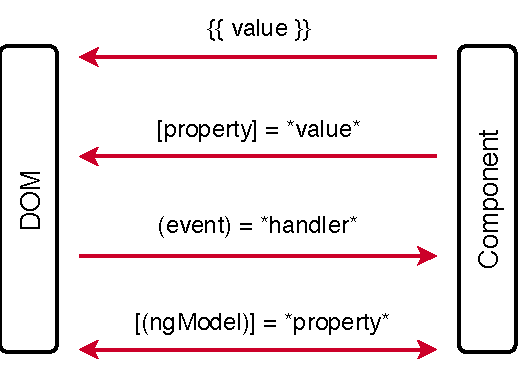
\includegraphics{gfx/DataBinding}
\caption[Flussrichtung der Daten bei \textit{Data-Binding}]{Flussrichtung der Daten bei \textit{Data-Binding}\cite{Data-Binding}}
\label{fig:technologies:databinding}
\end{figure}
\subsection{Observables}
\label{sec:technologies:angular:observables}
Bei Frontend-Frameworks wie Angular kommt es häufig vor, dass Daten über eine \acs{API} bezogen, verarbeitet und in die Seite eingebaut werden sollen. Das Verarbeiten der Daten kann dabei offensichtlich nur asynchron geschehen, also erst dann, wenn die Daten eintreffen und nicht, wenn die Methode zum Anfragen ausgeführt wird. Gleiches gilt beispielsweise auch für das Behandeln von \textit{Events} in Form von Benutzerinteraktionen. Hierfür werden bei Angular sogenannte \textit{Observables} verwendet, die Teil der Drittanbieter-Library \textit{RxJS} (Reactive Extensions for JavaScript) sind\cite{RxJS}.

Prinzipiell ist die asynchrone Ausführung von Code mittels \textit{Callback}-Methoden oder \textit{Promises} ebenso möglich. Der \acs{HTTP}-Client von Angular, mit dem der Datenaustausch mit einem Server organisiert wird, verwendet aber \textit{Observables}, welche auch sonst bei Angular gegenüber den Alternativen bevorzugt eingesetzt werden\cite{Observables}. Daher werdem diese hier näher erläutert. Beim \acs{HTTP}-Client ist es zwar nicht der Fall, ein \textit{Observable} kann aber im Allgemeinen seinen Zustand - also im Prinzip seinen Wert - über die Zeit ändern. Beispiel hierfür ist die Verarbeitung von Benutzereingaben. Generell ähnelt die Anwendung von \textit{Observables} der Nutzung der Events API; bei \textit{Observables} können allerdings \textit{Events} (bzw. deren Daten) bearbeitet werden, bevor sie an den eigentlichen \textit{Handler} weitergeleitet werden\cite{ObservableEvent}.

\begin{lstlisting}[float, floatplacement=h, style=htmlcssjs, caption={Beispiel für die Verwendung von \textit{Observables}}, label={Observables}]
@Injectable(/*...*/)
export class UserService {

  private url:string = ""; /*URL*/
  constructor(
    private http: HttpClient
  ) { }
  getUsers:Observable<User[]> {
    return this.http.get<User[]>(this.url);
  }
}
\end{lstlisting}
Wie ein \textit{Observable} genutzt werden kann, wird anhand der Datenübertragung mit dem \acs{HTTP}-Client von Angular in Beispiel \ref{Observables} demonstriert. In einem Service wird eine Methode definiert (Zeile 9), mit der eine Liste von Benutzern (also eine Array des Typs \textit{User}) über eine \acs{API} bezogen werden soll. Die \textit{get}-Methode des \acs{HTTP}-Client liefet ein Observable vom Typ \textit{User[]} zurück. Beim Aufruf dieser Methode in einer Komponente (Beispiel \ref{Subscriber}, Zeile 12) wird dann mit der \textit{subscribe}-Methode des zurückgegebenen \textit{Observable}-Objekts ein \textit{Subscriber} definiert. In diesem Fall ist dies eine Pfeilfunktion, in der die Antwort der Anfrage dem \textit{user}-Attribut der Komponente zugewiesen wird. Dieser \textit{Subscriber} wird logischerweise dann ausgeführt, wenn die Antwort vom Server eintrifft; der \textit{Subscriber} beobachtet also das \textit{Observable} bis es seinen Zustand ändert und wird dann ausgeführt. Dadurch, dass die Liste der Benutzer nach der Ausführung des \textit{Subscribers} dann nicht mehr leer ist, wird auch die Liste des Templates der Komponente (Zeile 15) angezeigt und darin dann die einzelnen Namen aufgelistet.

\begin{lstlisting}[float, floatplacement=h, style=htmlcssjs, caption={Beispiel für die Initialisierung eines \textit{Subscribers}}, label={Subscriber}]
@Component(
	template: '<ul *ngIf="users.length>0"><li *ng-for="let user of users">{{user.name}}</li></ul>'
[...])
export class UsersComponent implements OnInit {
  users: User[] = [];  
  
  constructor(
    private userService: UserService  
  ) { }
  
  onInit() {
    this.userService.getUsers()
      .subscribe(users => this.users = users)  
  }
}
\end{lstlisting}
\subsection{Routing}
\label{sec:technologies:angular:routing}
Das sogenannte \textit{Routing} ist eine elementarer Bestandteil bei \acfp{SPA}. Klickt man bei einer herkömmlichen Webseite auf einen Link, wird ein \acs{HTML}-Dokument angefordert, das entweder statisch ist oder - was häufiger der Fall ist - auf einem Server aus Datenbankeinträgen generiert wird. Im Falle einer \acs{SPA} werden nur ``rohe`` Daten - in der Regel im \acs{JSON}-Format oder als \acs{XML}-Datei angefragt und diese dann Client-seitig verarbeitet.  Abbildung \ref{fig:technologies:spa} illustriert den Unterschied zwischen herkömmliche Seiten und \acsp{SPA}.
\begin{figure}[h]
\centering
	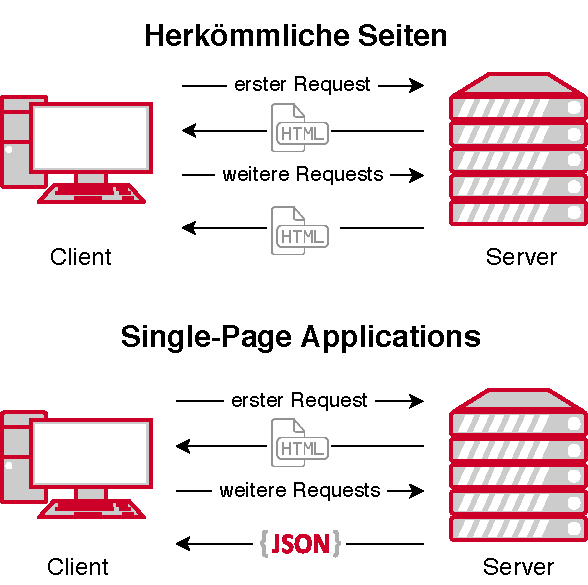
\includegraphics{gfx/SPA}
	\caption[Vergleich der Funktionsweise von herkömmlichen Seiten mit \textit{Single-Page Applications}]{Vergleich der Funktionsweise von herkömmlichen Seiten mit \textit{Single-Page Applications\cite{SPA}}}
	\label{fig:technologies:spa}
\end{figure}
Da bei normalen Webseiten für die Unterseiten oftmals der gleiche Kopf- und Fußbereich, gleiche Menüs oder Navigationsleisten sowie gleiche \textit{Stylesheets} für diese Bereiche verwendet werden, kann hier ein \textit{Overhead} vermieden werden, wenn beim Anklicken eines Links nur die Seitenbereiche geändert werden, die sich auch tatsächlich unterscheiden. Hierfür verhindert ein \textit{Router} beim Anklicken eines Link den \textit{Default} dieses Events, also das Anfragen eines neuen Dokuments und ``holt`` stattdessen Daten, beispielsweise von einer \acs{API}, die dann in ein Template eingesetzt werden, welches wiederum ins \acs{DOM} - also die Seite - eingebaut wird.

\begin{lstlisting}[float, floatplacement=h, style=htmlcssjs, caption={Beispiel eines  \textit{RouterModule}}, label={Routing}]
import { RouterModule, Routes } from '@angular/router';
import { UsersComponent } from 'users.component';

const routes: Routes = [
  {path: 'users', component: UsersComponent},
  {path: 'articles' loadChildren: './article.module#ArticleModule'},
  {path: '**', component: 404Component},
]
@ngModule(
  imports: [
    RouterModule.forRoot(routes)
  ],
  /*...*/
)
export class RouterModule {}
\end{lstlisting}
Code-Ausschnitt \ref{Routing} zeigt wie das Routing in Angular implementiert wird. In diesem Beispiel wurde dieses in ein eigenes Modul ausgelagert, es kann aber auch im \textit{Root Module} implementiert werden. Das Auslagern in ein eigenes Modul ist z.B. dann sinnvoll, wenn sehr viele Pfade und Komponenten verwaltet werden müssen. In diesem Fall muss dann das \textit{Routing Module} im \textit{Root Module} importiert werden. Ab Zeile 3 wird eine Liste von \textit{Routes} definiert, wobei einem Pfad eine Komponente zugeordnet wird, deren Template ins \acs{DOM} eingebaut werden soll, wenn der Pfad aufgerufen wird. Ein Pfad wird dabei einem HTML-Link-Tag (``a``) über das \textit{routerLink}-Attribut zugeordnet und nicht wie bei herkömmlichen Webseiten über das \textit{href}-Attribut.

Besucht man also die URL \textit{[\acs{FQDN}]/users} durch Eingabe in die Adressleiste des Browsers oder durch Anklicken eines entsprechenden Links, dann wird das Template der Komponente ``UsersComponent`` ins \acs{DOM} eingesetzt. Damit das funktioniert, muss im Template des \textit{Root Component} ein \textit{router-outlet}-Element eingefügt werden wie in Zeile 6 des Beispiels \ref{RoutingComponent}. Das Template der aktiven Komponente wird dann als Geschwister-Element dieses Elements ergänzt.
\begin{lstlisting}[float, floatplacement=h, style=htmlcssjs, caption={Beispiel eines Templates für das \textit{Root Component}, um Routing zu ermöglichen.\cite{RouterOutlet}}, label={RoutingComponent}]
<h1>Wilkommen</h1>
<nav>
  <a routerLink="/users">Benutzer</a>
  <a routerLink="/admin">Admin</a>
</nav>
<router-outlet></router-outlet>
\end{lstlisting}
Zeile 5 aus Beispiel \ref{Routing} zeigt zudem, wie \textit{Lazy Loading} implementiert wird. Erst wenn man die URL \textit{[\acs{FQDN}]/articles} besucht, wird das \textit{ArticleModule} nachgeladen, wobei dann in diesem weitere Pfade zu den Komponenten dieses Moduls analog zum \textit{Routing Module} definiert sein können. Soll weiterhin ein Artikel direkt über eine ID geöffnet werden können, muss in diesem untergeordneten Modul ein Pfad `:id` definiert sein, sodass beim Aufruf von \textit{[\acs{FQDN}]/articles/1} der Artikel mit der ID `1` angezeigt werden kann. In Kapitel \ref{sec:prog:searchPerson} wird hiervon Gebrauch gemacht.

Will man die Seite in mehrere Module unterteilen, ohne dass diese nachgeladen werden müssen, so kann man beim Importieren des \textit{RouterModule} (Beispiel\ref{Routing}, Zeile 10) die Option \texttt{\{'preloadStrategy: PreloadAllModules'\}} mitgeben. Dadurch werden beim ersten Seitenaufruf alle Module auf einmal geladen. Bei großen Modulen kann das allerdings entsprechend lang dauern.

\subsection{Zusammenfassung der Architektur}
\label{sec:technologies:angular:architecture}

\begin{figure}[h]
\centering
	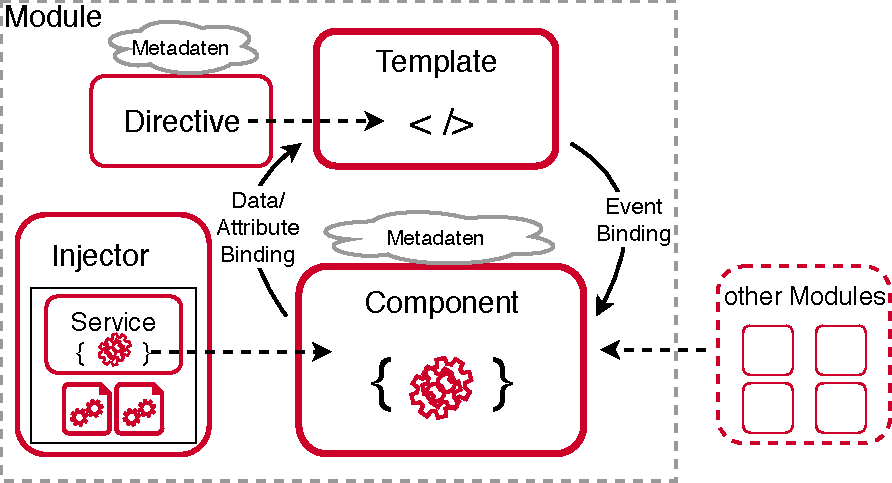
\includegraphics{gfx/Architektur}
	\caption[Übersicht über die Architektur des Angular-Frameworks]{Übersicht über die Architektur des Angular-Frameworks\cite{Architecture}}
	\label{fig:technologies:angular:architecture}
\end{figure}

Aus den bisher vorgestellten Bausteinen von Angular lässt sich eine grobe Architektur ableiten, die in Abbildung \ref{fig:technologies:angular:architecture} dargestellt ist. Komponenten sind die Kernbausteine und in Modulen zusammengefasst, wobei die Metadaten der Komponenten Informationen über das zugehörige Template, CSS-Regeln, Services etc. enthält. Über Services, die in das Modul oder die Komponenten ''injiziert'' werden, können letztere Daten von einem Server oder anderen Komponenten beziehen. Diese Daten können mittels \textit{Data Binding} oder \textit{Attribute Binding} in dem zur Komponente gehörenden Template unter Zuhilfenahme von Direktiven eingebunden werden. Umgekehrt kann mit \textit{Event Bindings} auf Benutzerinteraktionen reagiert und der Zustand der Komponente geändert werden. Außerdem können andere Module importiert und somit deren Funktionalitäten genutzt werden. Darüber hinaus kann mittels \textit{Routing} das Navigieren zwischen Seiten simuliert werden, indem Templates verschiedener Komponenten gegeneinander ausgetauscht werden.

\subsection{Das Befehlszeilen-Interface (CLI)}
\label{sec:technologies:angular:cli}
Mit der Version 2 von Angular - also der grundlegenden Überarbeitung - wurde für dieses Framework das Paket @angular/cli veröffentlich, welches ein Befehlszeilen-Interface enthält. Dieses \acs{CLI} soll die Entwicklung mit Angular vereinfachen und enthält im wesentlichen Befehle für:

\begin{itemize}
\item das Erzeugen einer neuen Anwendung
\item das Generieren von \textit{ngModules}, \textit{Components}, \textit{Services} etc.
\item das Hinzufügen und Installieren zusätzlicher Pakete
\item das Testen und ``Zusammenbauen`` der Anwendung
\end{itemize}

Dieses Befehlszeilen-Interface wird über den Paketmanager \textit{npm} bezogen, über den bei Erzeugung eines neuen Projektes mit dem Befehl \textit{ng new} zusätzliche Pakete installiert werden, die für eine rudimentäre, auf Angular basierende, Webanwendung notwendig sind. Außerdem können mit \textit{npm} dem Projekt im Verlauf der Entwicklung weitere Pakete und Software-Bibliotheken hinzugefügt werden.

Der Befehl \textit{ng generate} (oder kurz \textit{ng g}) bietet Optionen zum Generieren generischer Klassen und Interfaces, aber auch zum Erzeugen Angular-spezifischer Klassen wie \textit{Components, ngModules, Services} etc. Bei der Generierung einer Angular-spezifischen Klasse wird neben der eigentlichen Datei, in der diese Klasse implementiert wird, eine weitere Datei erstellt, in der sich ein Gerüst für \textit{Unit-Tests} der Klasse befindet. Im Falle einer Komponente werden diese Dateien in einem Ordner, der den gleichen Namen wie die Komponente hat, erzeugt und in diesem außerdem jeweils eine Datei für das zugehörige \acs{HTML}-Template (\ref{sec:technologies:angular:component:html}) sowie für die \acs{CSS}-Regeln (\ref{sec:technologies:angular:component:css}) erstellt - insgesamt also 4 Dateien. Allerdings kann über eine \textit{Flag} erreicht werden, dass statt einer eigenen Datei für das Template ein Inline-Template in der \textit{.component.ts}-Datei erstellt wird. Außerdem wird die Komponente dem \textit{declarations}-Array des - auf die Ordnerhierarchie bezogen - nächstgelegenen Moduls hinzugefügt (vgl. \ref{sec:technologies:angular:module}). Dies gilt auch für das Erzeugen von Direktiven, Services und Pipes.

Am Anfang von Kapitel \ref{sec:technologies:angular} wurde der Befehl \textit{ng add} bereits oberflächlich vorgestellt. Im Unterschied zum Ergänzen neuer Pakete via \textit{npm} werden bei Benutzung dieses Befehls die Pakete dem Projekt nicht einfach nur hinzugefügt, sondern sie können direkt über ein Installationsskript in das Projekt eingebunden werden.

Weiterhin wichtig sind die Befehle \textit{ng test}, mit dem die Unit-Tests gestartet werden können, und \textit{ng serve}, durch welchen ein Entwicklungsserver gestartet wird, mit dem standardmäßig die Webanwendung neu geladen wird, wenn Dateien bearbeitet wurden. Hierfür wird die \textit{NodeJS}-Umgebung genutzt.

Zuletzt gibt es noch den Befehl \textit{ng build}, mit dem die Webanwendung für die Auslieferung auf einen Server vorbereitet wird: Dafür wird beispielsweise TypeScript in JavaScript übersetzt oder Dateien werden komprimiert.

\section{TypeScript}
\label{sec:technologies:ts}
TypeScript ist eine quelloffene, von Microsoft entwickelte Programmiersprache, welche ein \textit{Superset} von JavaScript darstellt. Hauptmerkmal von TypeScript ist, dass es im Gegensatz zu JavaScript die Möglichkeit bietet, statische Typen zu nutzen. Als primitive Typen gibt es \textit{number}, die immer als Fließkommazahl gespeichert werden und auch für binäre, oktale und hexadezimale Literale genutzt werden können, und \textit{string}. Ebenso gibt es Arrays ebendieser\cite{Types}. Damit können dann natürlich auch typisierte Klassen entwickelt werden. Außerdem ergänzt es JavaScript um weitere Funktionalitäten wie \textit{Namespaces}, also Namensräume oder \textit{Interfaces}. Mit einem Compiler, der mit dem Paketverwaltungssystem \textit{npm} installiert werden kann, muss TypeScript vor der Auslieferung in JavaScript übersetzt werden\cite{TypeScript}. TypeScript hilft also dabei, Code zu entwickeln bei dem die einzelnen Teile wirklich zueinander passen und nicht beispielsweise ein Methodenaufruf  mit falschen Parametern erfolgt. Somit können Laufzeitfehler minimiert bzw. weitestgehend vermieden werden.

Da JavaScript-Code prinzipiell auch TypeScript-Code ist, können JavaScript-Bibliotheken auch in TypeScript verwendet werden. Diese Bibliotheken sind dann allerdings zunächst ``untypisiert``. Über das Projekt \textit{Definitely Typed} (\href{https://definitelytyped.org/}{https://definitelytyped.org/}) können für sehr viele JavaScript-Bibliotheken sogenannte \textit{Type Definitions} bezogen und mittels \textit{npm} installiert werden. Somit kann dann die Bibliothek ``typisiert`` genutzt werden. Diese muss dabei natürlich trotzdem im Projekt vorhanden sein, sie wird fortan lediglich indirekt genutzt.
\section{Sonstiges}
\label{sec:technologies:other}

\paragraph*{OpenLayers}
\label{sec:technologies:ol}
Bei OpenLayers handelt es sich um eine Library, mit der Karten in Webseiten eingebunden werden können. Dabei kann Kartenmaterial verschiedenster Quellen genutzt werden; am häufigsten wird OpenStreetMap verwendet, aber auch andere Quellen sind möglich. Die \acs{API} dieser Library bietet zahlreiche Möglichkeiten, um das verwendete Kartenmaterial zu manipulieren oder zusätzliche Informationen auf der Karte einzublenden. Diese Library ist ein unter der \textit{2-Klausel-BSD}-Lizenz veröffentlichtes Open Source-Projekt\cite{OpenLayers}.

\paragraph*{angular-oauth2-oidc}
\label{sec:technologies:oidc}
Das Paket \textit{angular-oauth2-oidc} ermöglicht die Authentifizierung eines Benutzers über die OpenID Connect-Authentifizierungsschicht. Nachdem in einer \acs{JSON}-Datei konfigurt wurde, welcher \textit{Identity-Provider} verwendet werden soll (sprich: zu welcher Seite er weitergeleitet wird, um sich dort zu authentifizieren), kann eingestellt werden, dass der Nutzer direkt beim initialen Seitenaufruf zum Login-Portal weitergleitet werden soll, oder ob dies erst geschieht, wenn auf einen dedizierten Login-Button geklickt wird. Hat sich der Benutzer erfolgreich eingeloggt, kann ein vom \textit{Identity Provider} bereitgestelltes Token zum Header von Anfragen, die einer Authentifizierung bedürfen, hinzugefügt werden. Dieses Paket wurde unter der MIT-Lizenz veröffentlicht und ist damit Open Source-Software\cite{oidc}.

\paragraph*{ngx-barcode}
\label{sec:technologies:barcode}
Dieses Paket ergänzt Angular um eine Komponente, mit der Barcodes in verschiedenen Formaten dargestellt werden können. Auch dieses Paket wurde unter der MIT-Lizenz veröffentlicht\cite{barcode}.

\paragraph*{Angular Material (@angular/material)}
\label{sec:technologies:material}
Das vom Angular-Team entwickelte Paket \textit{@angular/material} (https://material.angular.io) bietet eine ganze Reihe an Komponenten für die Gestaltung des Aufbaus einer Webseite. Zu diesen Komponenten zählen beispielsweise Listen, Formularfelder oder Menüs. Dabei ist das Design aller Komponenten dem von Google entwickelten \textit{Material Design} nachempfunden. Dieses zeichnet sich durch flache Elemente und kontrastreiche Farben aus. Mit diesem Paket ist es möglich, eine mit dem Angular-Framework entwickelte Webanwendung anspruchsvoll zu gestalten, ohne selbst (viel) \acs{CSS} schreiben zu müssen. Dieses Paket ist dabei abhängig von den Paketen @angular/animations (für Animationen) und @angular/cdk, dem \textit{Component Development Kit}. Letzteres hilft beispielsweise beim Entwickeln von Overlays oder bei der barrierefreien Gestaltung.

\paragraph*{Angular Progressive Web App (@angular/pwa)}
\label{sec:technologies:angular/pwa}
Mit diesem Paket, kann eine Angular-App ganz einfach in eine \textit{\acl{PWA}} verwandelt werden, indem dem Projekt eine Manifest-Datei, ein \textit{Service Worker}-Skript und eine Konfigurationsdatei hinzugefügt werden. Damit nimmt einem dieses Paket viel Arbeit ab, weil die Implementierung des Service Workers sowie dessen Registrierung und Installation im Browser durch dieses Paket übernommen werden. Damit verbleibt nur, in der Konfigurationsdatei die Ressourcen, welche im Cache gespeichert werden sollen, zu definieren.

\paragraph*{Material Design Icons}
\label{sec:technologies:Mat-Icons}
Bei \textit{Material Design Icons} (https://materialdesignicons.com/) handelt es sich um ein Projekt, über das unzählige Icons im Stile des Material Designs in verschiedenen Formaten (als .png- oder .svg-Datei oder als Font) bereitgestellt werden. Bei diesen Icons handelt es sich zum Teil um von Google selbst entworfene (und in dessen Projekten genutzte) Bilder, zum Großteil aber um Graphiken, die von Dritten eingereicht wurden; man kann also auch selbst welche vorschlagen.

\paragraph*{Icons8}
\label{sec:technologies:icons8}
Im Gegensatz zu den Icons von \textit{Material Design Icons} sind die bei Icons8 (https://icons8.de) erhältlichen Graphiken nicht (nur) monochrom, sondern mehrfarbig verfügbar. Diese sind zwar prinzipiell auch kostenlos erhältlich, dann allerdings nicht in allen Auflösungen und nur als .png-Datei. Vollumfänglicher Zugriff auf diese kann mit dem Erwerb einer Lizenz erhalten werden, außerdem erhält man so Zugriff auf weitere Funktionen.


\paragraph*{Bilder}
\label{sec:technologies:Images}
Das für diese Webanwendung verwendete Hintergrundbild stammt von \href{https://www.pexels.com}{https://www.pexels.com}.
